\chapter{Descripción de la propuesta}
\label{cap:descripcion_propuesta}

El presente capítulo expone el diseño formal, la descomposición modular y la especificación de ingeniería de software de la plataforma desarrollada para la automatización del modelado dinámico e interpretable de estudiantes en Entornos Virtuales de Aprendizaje (LMS). A diferencia de las soluciones convencionales reportadas en la literatura que procesan bitácoras de manera estática o retrospectiva, la propuesta materializa una infraestructura basada en eventos capaz de inferir la evolución del comportamiento del usuario en tiempo de ejecución, preservando la transparencia algorítmica indispensable para la toma de decisiones docentes.

\section{Diseño general de la solución o modelo}
\label{sec:diseno_general}

Para superar las restricciones inherentes al procesamiento analítico por lotes (\textit{batch}) en entornos educativos, el diseño conceptual del sistema se fundamenta en los postulados de la \textbf{Arquitectura Kappa}. Este paradigma de ingeniería de datos postula que todo procesamiento computacional—tanto histórico como en tiempo real—puede unificarse a través de un único flujo continuo de eventos inmutables. En el contexto de los Sistemas de Gestión de Aprendizaje (LMS), donde las interacciones de los estudiantes ocurren de forma concurrente y no determinista, la arquitectura Kappa desacopla la captura de eventos de la inferencia analítica, garantizando un rendimiento con latencias del orden de milisegundos y eliminando la duplicidad lógica característica de las arquitecturas Lambda.

\subsection{Arquitectura en capas y desacoplamiento de componentes}

La solución propuesta articula cinco capas funcionales orquestadas sobre una infraestructura de contenedores aislados, garantizando la escalabilidad horizontal, la tolerancia a fallos y la portabilidad del sistema en despliegues institucionales. En la Figura~\ref{fig:diagrama_arquitectura} se ilustra la topología general de la arquitectura y las dependencias de comunicación entre subsistemas.

\begin{figure}[H]
    \centering
    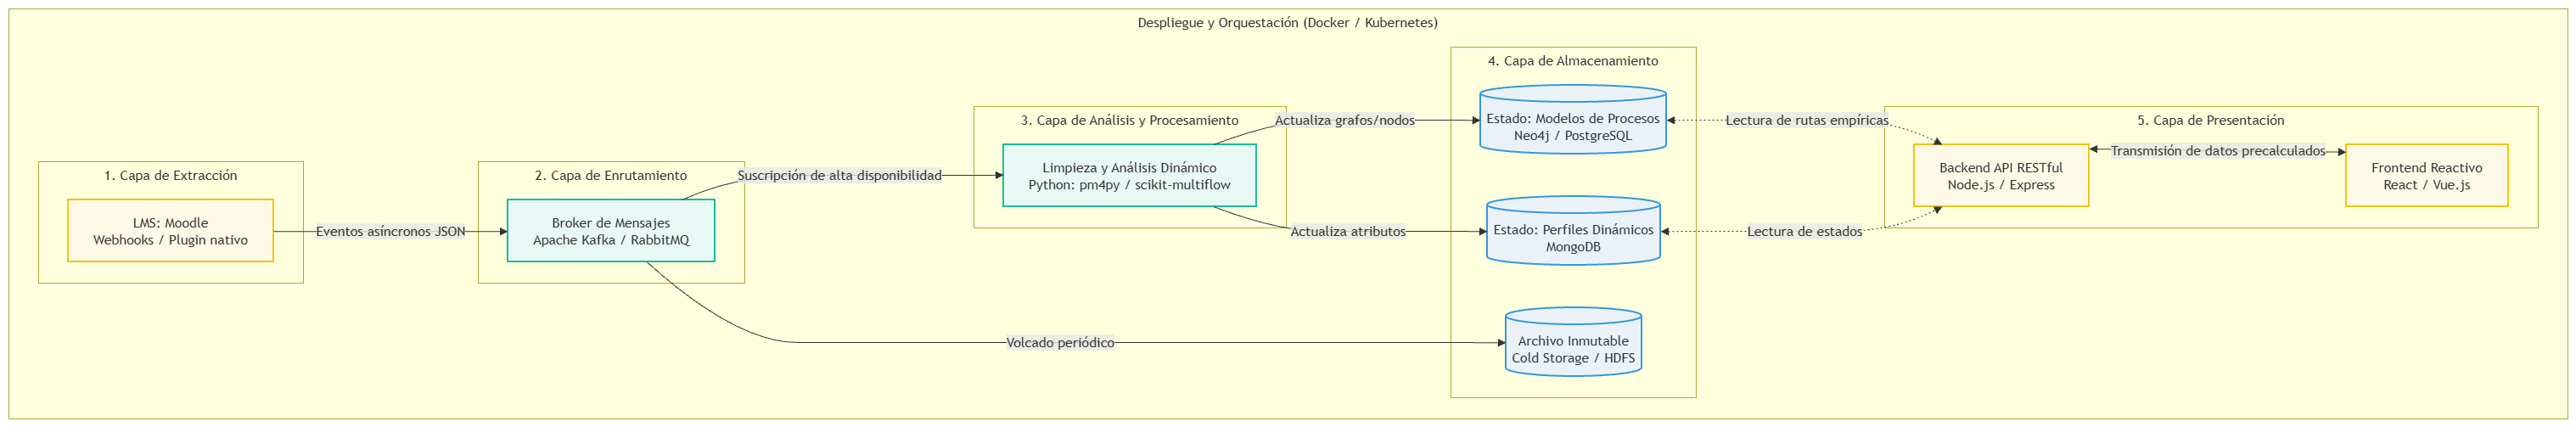
\includegraphics[width=\textwidth]{figuras/diagrama_arquitectura.png}
    \caption{Topología del sistema basada en la Arquitectura Kappa para el procesamiento continuo de eventos de interacción en LMS.}
    \label{fig:diagrama_arquitectura}
    \fuente{Elaboración propia.}
\end{figure}

A nivel estructural, la arquitectura se delimita mediante las siguientes responsabilidades de diseño:

\begin{itemize}
    \item \textbf{Capa de Extracción (Ingesta):} Encargada de capturar los eventos elementales de navegación, clics y envíos evaluativos generados por los estudiantes dentro del LMS Moodle. La captura opera de forma no intrusiva mediante \textit{webhooks} asíncronos y componentes de extensión nativos, evitando sobrecargar la base de datos transaccional de la plataforma educativa.
    
    \item \textbf{Capa de Enrutamiento y Mensajería:} Implementa un intermediario de mensajes distribuido (\textit{message broker}) de alta concurrencia (como Apache Kafka o RabbitMQ). Actúa como un búfer transitorio inmutable que garantiza tolerancia a picos masivos de tráfico concurrente, preservando el orden secuencial estricto de las trazas estudiantiles antes de su procesamiento.
    
    \item \textbf{Capa de Análisis y Procesamiento Dinámico:} Constituye el núcleo computacional de la plataforma. Este componente suscribe los eventos del intermediario para aplicar transformaciones de reducción de ruido, extracción de características y ejecución paralela de algoritmos de minería de flujos (\textit{stream clustering}) y minería de procesos educativos (\textit{Educational Process Mining}, EPM).
    
    \item \textbf{Capa de Almacenamiento Políglota:} Diseñada bajo un esquema heterogéneo que atiende diferentes naturalezas de acceso a datos:
    \begin{itemize}
        \item \textit{Archivo Inmutable (Cold Storage):} Persiste la totalidad de eventos crudos en almacenamiento distribuido o en bloque (e.g., HDFS o volúmenes montados), garantizando la auditabilidad y reproducibilidad experimental de los modelos.
        \item \textit{Estado de Perfiles Dinámicos:} Base de datos NoSQL documental (MongoDB) que resguarda el estado actual de cada estudiante mediante objetos JSON polimórficos que mutan incrementalmente.
        \item \textit{Estado de Modelos de Procesos:} Base de datos relacional o grafo (PostgreSQL/Neo4j) que almacena la topología de los Grafos de Dependencia Directa (\textit{Directly-Follows Graphs}, DFG) descubiertos.
    \end{itemize}
    
    \item \textbf{Capa de Presentación e Interpretabilidad:} Interfaz reactiva (SPA en React o Vue.js) desacoplada mediante una API RESTful asíncrona (Node.js/Express). Proporciona a los educadores tableros visuales interactivos de ``caja blanca'', permitiendo auditar la trayectoria empírica que justifica la pertenencia de un estudiante a un clúster determinado.
\end{itemize}

\subsection{Modelo temporal y dinámica de tuberías de datos}

El flujo operativo que gobierna la sincronía del sistema se descompone en cuatro tuberías de procesamiento continuo (\textit{pipelines}). En la Figura~\ref{fig:diagrama_secuencia} se detalla la secuencia temporal asíncrona, desde el instante en que el alumno interactúa en la plataforma educativa hasta que el docente visualiza el modelo actualizado.

\begin{figure}[H]
    \centering
    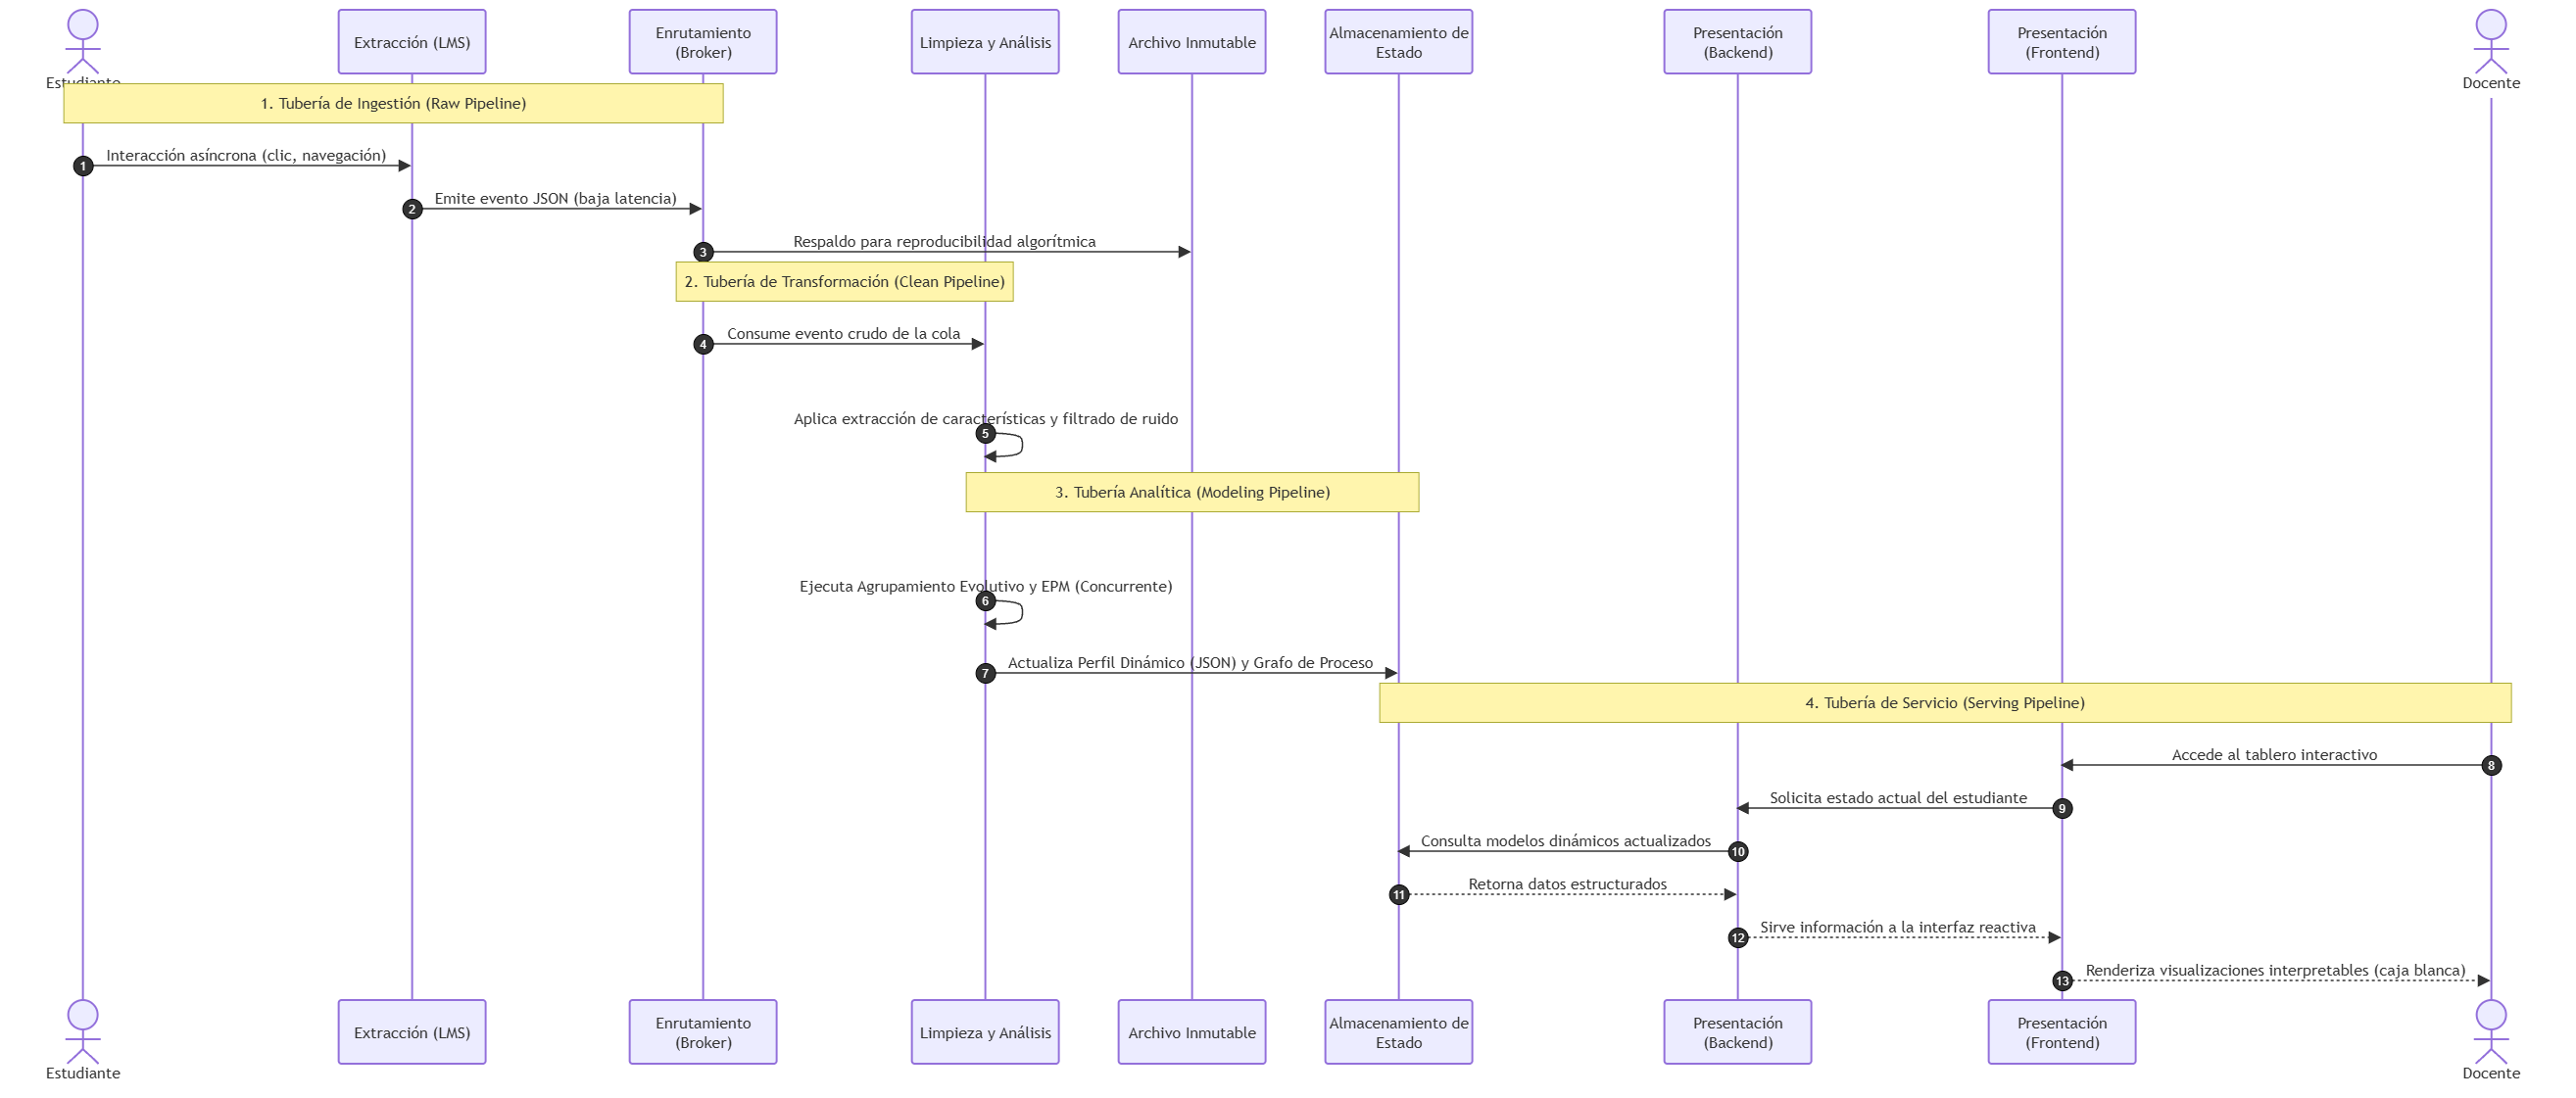
\includegraphics[width=\textwidth]{figuras/diagrama_secuencia.png}
    \caption{Diagrama de secuencia de la interacción asíncrona a través de las cuatro tuberías de procesamiento de la arquitectura.}
    \label{fig:diagrama_secuencia}
    \fuente{Elaboración propia.}
\end{figure}

El ciclo analítico opera de forma continua y coordinada mediante las siguientes fases:

\begin{enumerate}
    \item \textbf{Tubería de Ingestión (\textit{Raw Pipeline}):} Captura las interacciones asíncronas generadas por el estudiante en Moodle y emite inmediatamente un mensaje estructurado en formato JSON hacia la cola del intermediario de mensajes (\textit{broker}). Esta transacción se ejecuta de manera no bloqueante para asegurar un impacto nulo en la experiencia de usuario del LMS. Simultáneamente, el intermediario vuelca una réplica inmutable al archivo de almacenamiento en frío para salvaguardar la consistencia de los datos.
    
    \item \textbf{Tubería de Transformación (\textit{Clean Pipeline}):} El procesador de flujos consume los eventos crudos encolados, realiza la imputación o descarte de anomalías temporales y aplica filtros para eliminar eventos irrelevantes del sistema (e.g., consultas repetitivas de sesión o peticiones de recursos estáticos). Asimismo, abstrae las acciones elementales hacia Eventos de Alto Nivel (\textit{High-Level Events}), consolidando las matrices de atributos requeridas por los modelos computacionales.
    
    \item \textbf{Tubería Analítica (\textit{Modeling Pipeline}):} Los eventos transformados alimentan en tiempo real y de forma concurrente dos componentes analíticos:
    \begin{itemize}
        \item El motor de agrupamiento evolutivo sobre flujos continuos ajusta los centroides de los perfiles estudiantiles sin reiniciar el cómputo sobre el historial acumulado.
        \item El algoritmo de minería de procesos educativos registra las transiciones de estados para reconfigurar el Grafo de Dependencia Directa correspondiente a la ruta de navegación real del estudiante.
    \end{itemize}
    Una vez procesado el evento, la tubería actualiza atómicamente el documento del perfil en MongoDB y los nodos del grafo en el almacén de procesos.
    
    \item \textbf{Tubería de Servicio y Visualización (\textit{Serving Pipeline}):} Cuando el educador ingresa al tablero analítico, la interfaz gráfica consulta a la API RESTful el estado actual precalculado. El servicio despacha las estructuras de datos cacheadas directamente desde el almacén de estado, eliminando tiempos de espera analíticos y renderizando de manera reactiva representaciones transparentes de los patrones formativos.
\end{enumerate}